\documentclass[../thesis/thesis.tex]{subfiles}
\begin{document}
 \chapter{Orphans: Node Structure}

\section{Node Hardware}
 
\begin{figure}
\centering
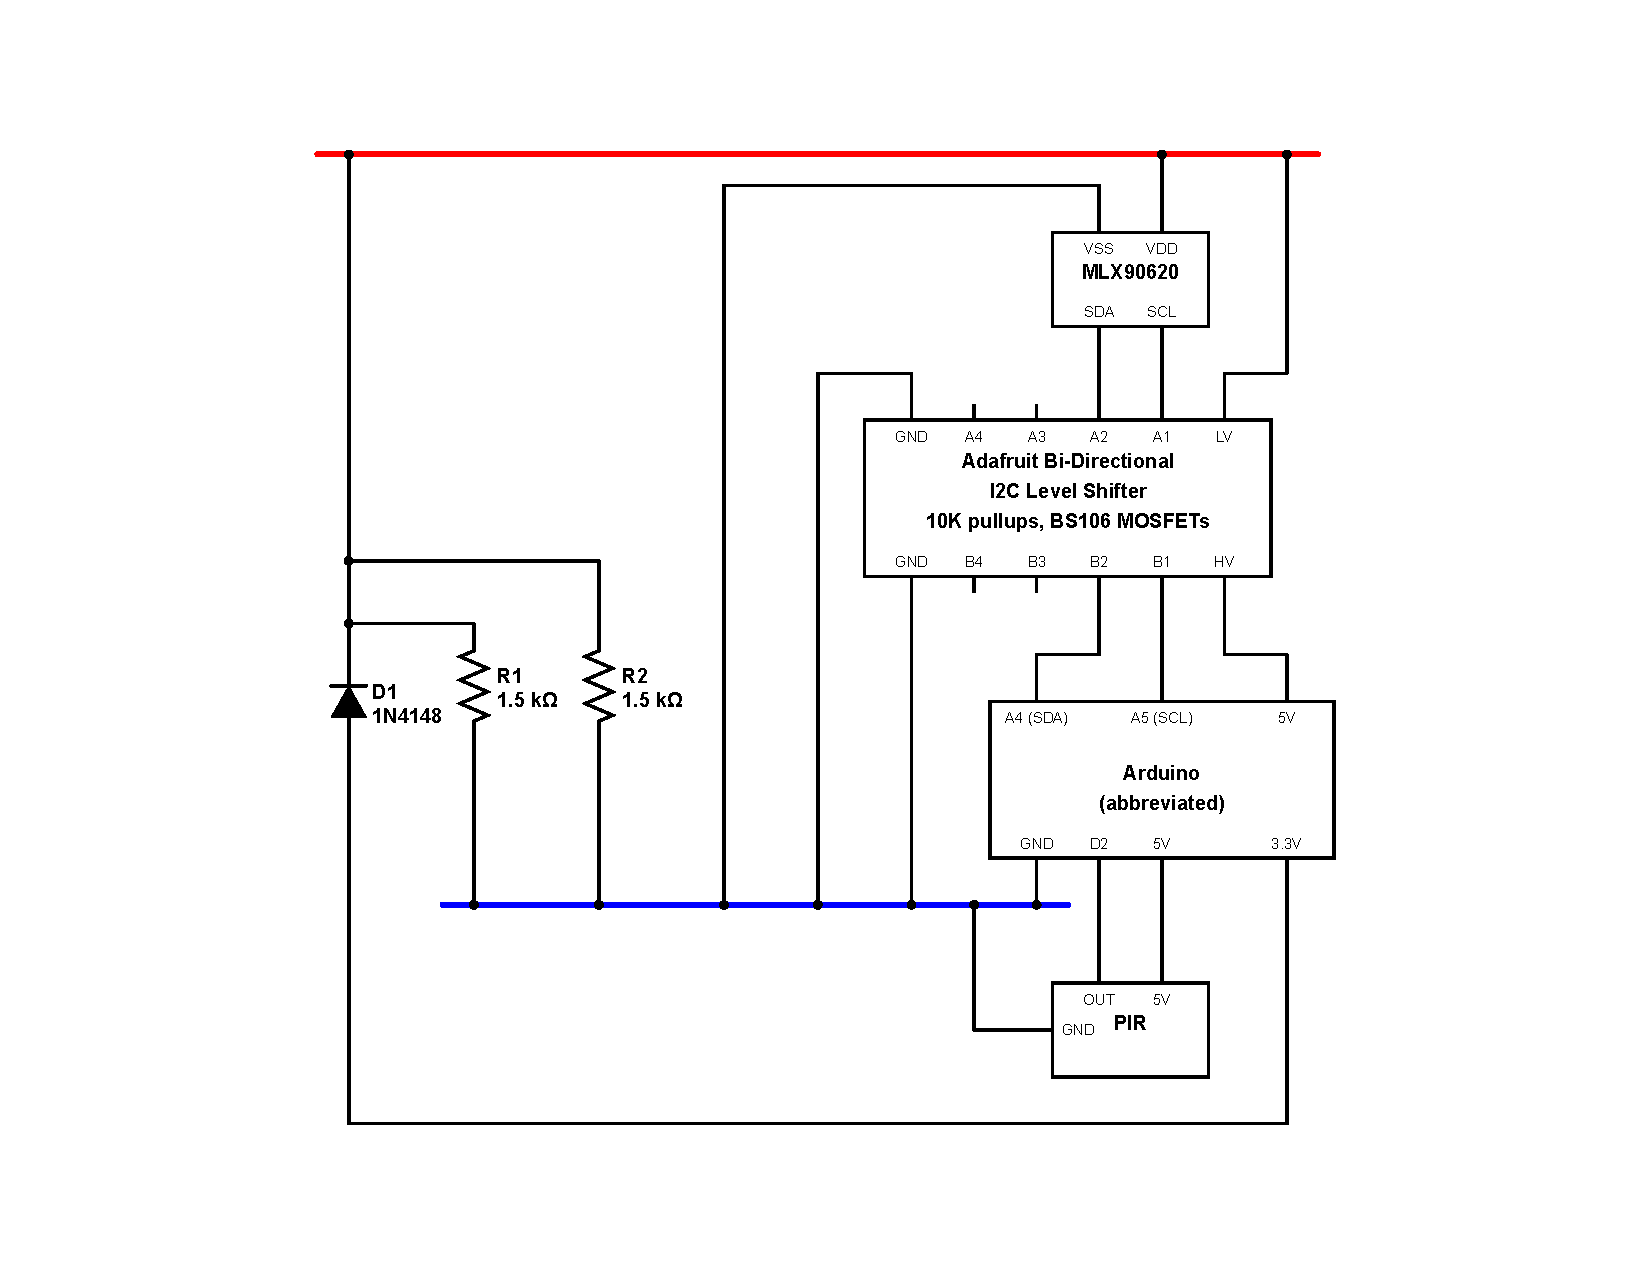
\includegraphics[width=\textwidth]{../diagrams/mlx-arduino.pdf}
\caption{MLX90620, PIR and Arduino integration circuit}
\label{fig:circuits:node}
\end{figure}

Due to low cost and ease of use, the \ard platform was selected as the host for the low-level \iic interface for communication to the \mlx. Initially, this presented some challenges, as the \mlx recommends a power and communication voltage of 2.6V, while the \ard is only able to output 3.3V and 5V as power, and 5V as communication. Due to this, it was not possible to directly connect the \ard to the \mlx, and similarly due to the two-way nature of the \iic 2-wire communication protocol, it was also not possible to simply lower the \ard voltage using simple electrical techniques, as such techniques would interfere with two-way communication.

A solution was found in the form of a \iic level-shifter, the Adafruit ``4-channel I2C-safe Bi-directional Logic Level Converter'' \cite{AdafruitI2C}, which provided a cheap method to bi-directionally communicate between the two devices at their own preferred voltages. The layout of the circuit necessary to link the \ard and the \mlx using this converter can be seen in \Fref{fig:circuits:node}.

Additionally, as used in the Thermosense paper, a \pir motion sensor \cite{AdafruitPIR} was also connected to the \ard. This sensor, operating at 5V natively, did not require any complex circuitry to interface with the \ard. It is connected to digital pin 2 on the \ard, where it provides a rising signal in the event that motion is detected, which can be configured to cause an interrupt on the \ard. In the configuration used in this project, the sensor's sensitivity was set to the highest value (TODO: check) and the timeout for re-triggering was set to the lowest value (approximately 2.5 seconds). Additionally, the continuous re-triggering feature (whereby the sensor produces continuous rising and falling signals for the duration of motion) was disabled using the provided jumpers. 

\section{Node Software}

To calculate the final temperature values that the \mlx offers, a complex initialisation and computational process must be followed, which is specified in the sensor's datasheet \cite{MLXDatasheet}. This process involves initialising the sensor with values attained from a separate on-board \iic EEPROM, then retrieving a variety of normalisation and adjustment values, along with the raw sensor data, to compute the final temperature result.

The basic algorithm to perform this normalisation was based upon code by users ``maxbot'', ``IIBaboomba'', ``nseidle'' and others on the Arduino Forums \cite{ArduinoForum} and was modified to operate with the newer \ard ``Wire'' \iic libraries released since the authors' posts. In pursuit of the project's aims to create a more approachable thermal sensor, the code was also restructured and rewritten to be both more readable, and to introduce a set of features to make the management of the sensor data easier for the user, and for the information to be more human readable.

The first of the features introduced was the human-readable format for serial transmission. This allows the user to both easily write code that can parse the serial to acquire the serial data, as well as examine the serial data directly with ease. When the \ard first boots running the software, the output in \Fref{fig:code:initseq} is output. This specifies several things that are useful to the user; the attached sensor (``DRIVER''), the build of the software (``BUILD'') and the refresh rate of the sensor (``IRHZ''). Several different headers, such as ``ACTIVE'' and ``INIT'' specify the current millisecond time of the processor, thus indicating how long the execution of the initialisation process took (33 milliseconds).

Once booted, the user is able to send several one-character commands to the sensor to configure operation, which are described in \Fref{tab:ardcommands}. Depending on the sensor configuration, IR data may be periodically output automatically, or otherwise manually triggered. This IR data is produced in the packet format described in \Fref{fig:code:packet}. This is a simple, human readable format that includes the millisecond time of the processor at the start and end of the calculation, if the \pir has seen any motion for the duration of the calculation, and the 16x4 grid of calculated temperature values.

\begin{figure}
 \centering
\begin{lstlisting}[style=arduino]
INIT 0
INFO START
DRIVER MLX90620
BUILD Feb  1 2015 00:00:00
IRHZ 1
INFO STOP
ACTIVE 33
\end{lstlisting}
\caption{Initialisation sequence}
\label{fig:code:initseq}
\end{figure}

\begin{table}
\centering
\begin{tabular}{|l|l|}
\hline
\texttt{R} & Flush buffers and reset \ard \\ \hline
\texttt{I} & Print INFO again \\ \hline
\texttt{T} & Activate timers for periodic IR data output \\ \hline
\texttt{O} & Deactivate timers for periodic IR data output \\ \hline
\texttt{P} & Manually trigger capture and output of IR data \\ \hline
\texttt{F\textit{x}} & Set sensor refresh frequency to \textit{x} and reboot \\ \hline
\end{tabular}
\caption{Commands}
\label{tab:ardcommands}
\end{table}

\begin{figure}
 \centering
\begin{lstlisting}[style=arduino]
START 34
MOVEMENT 0
1.0  1.0  1.0  1.0  1.0  1.0  1.0  1.0  1.0  1.0  1.0  1.0  1.0  1.0  1.0  1.0
1.0  1.0  1.0  1.0  1.0  1.0  1.0  1.0  1.0  1.0  1.0  1.0  1.0  1.0  1.0  1.0
1.0  1.0  1.0  1.0  1.0  1.0  1.0  1.0  1.0  1.0  1.0  1.0  1.0  1.0  1.0  1.0
1.0  1.0  1.0  1.0  1.0  1.0  1.0  1.0  1.0  1.0  1.0  1.0  1.0  1.0  1.0  1.0
STOP 97
\end{lstlisting}
\caption{Thermal data packet}
\label{fig:code:packet}
\end{figure}

\begin{figure}
\centering
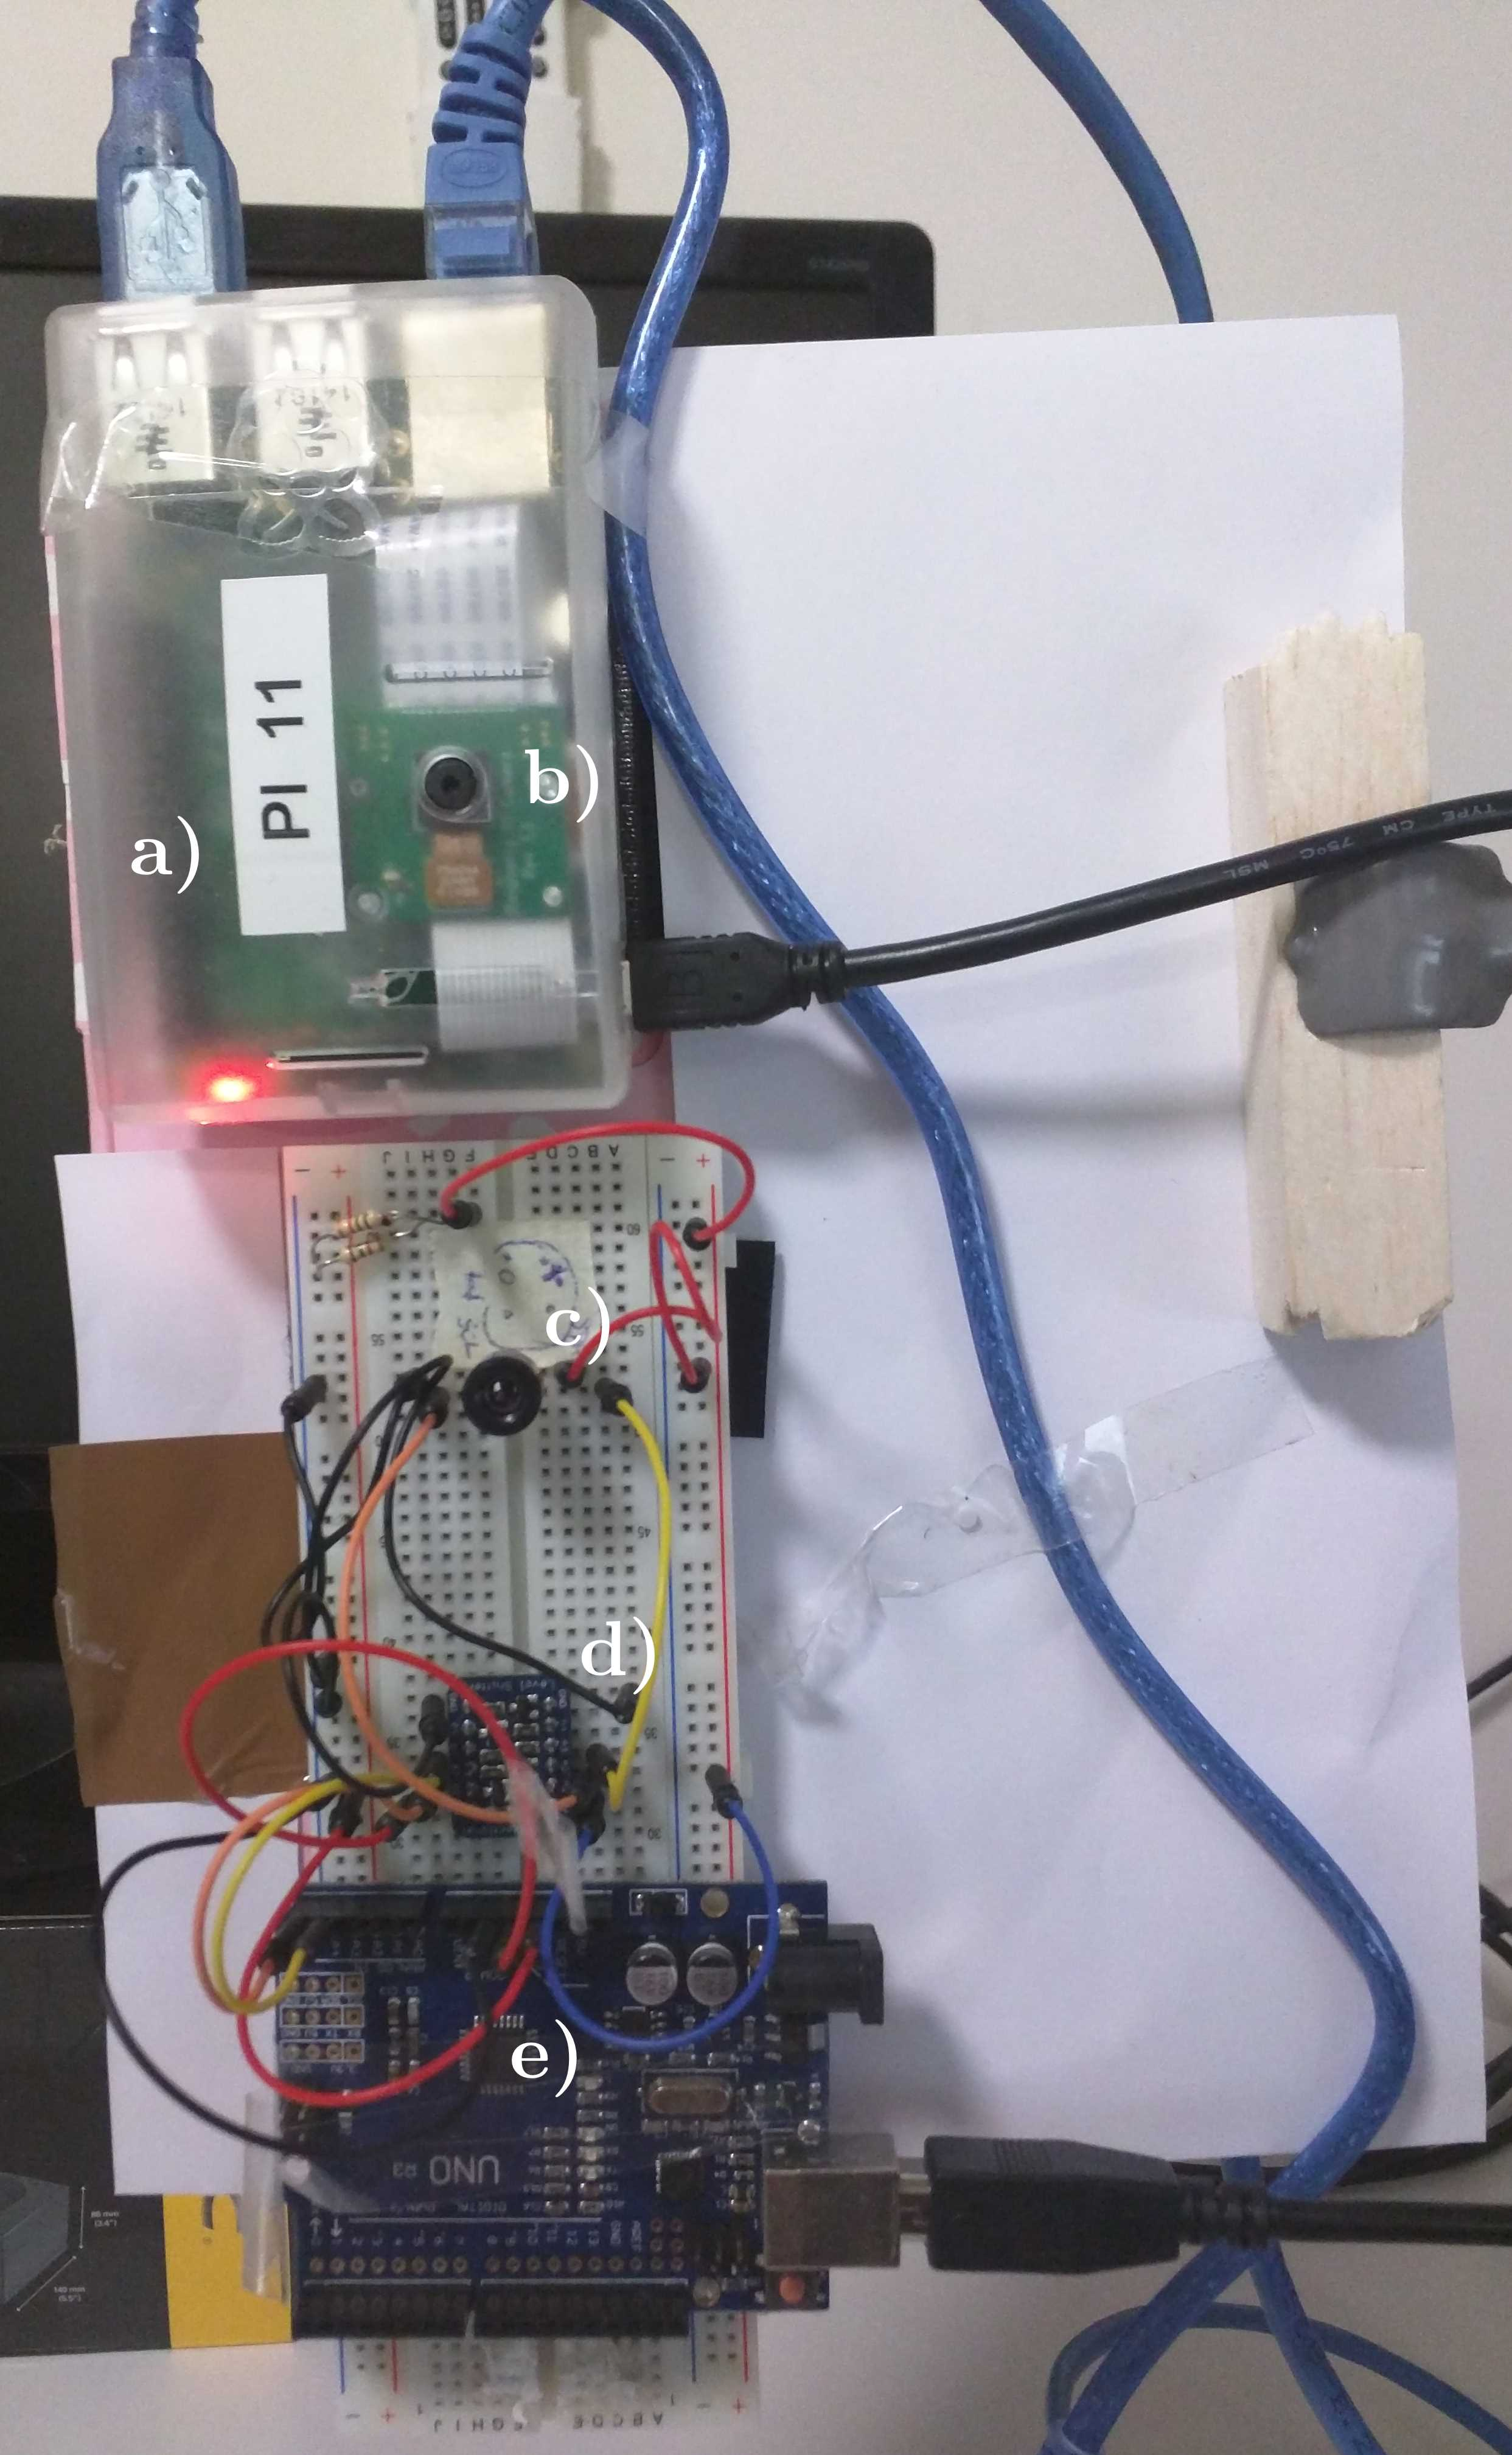
\includegraphics[height=0.7\textheight]{../diagrams/prototypea.jpg}
{\small
\begin{enumerate}[a)]
 \item Raspberry Pi
 \item Camera
 \item \mlx
 \item Level-shifting circuitry
 \item Arduino
\end{enumerate}
}
\caption{Prototype A}
\label{fig:pictures:protoa}
\end{figure}

\begin{figure}
\centering
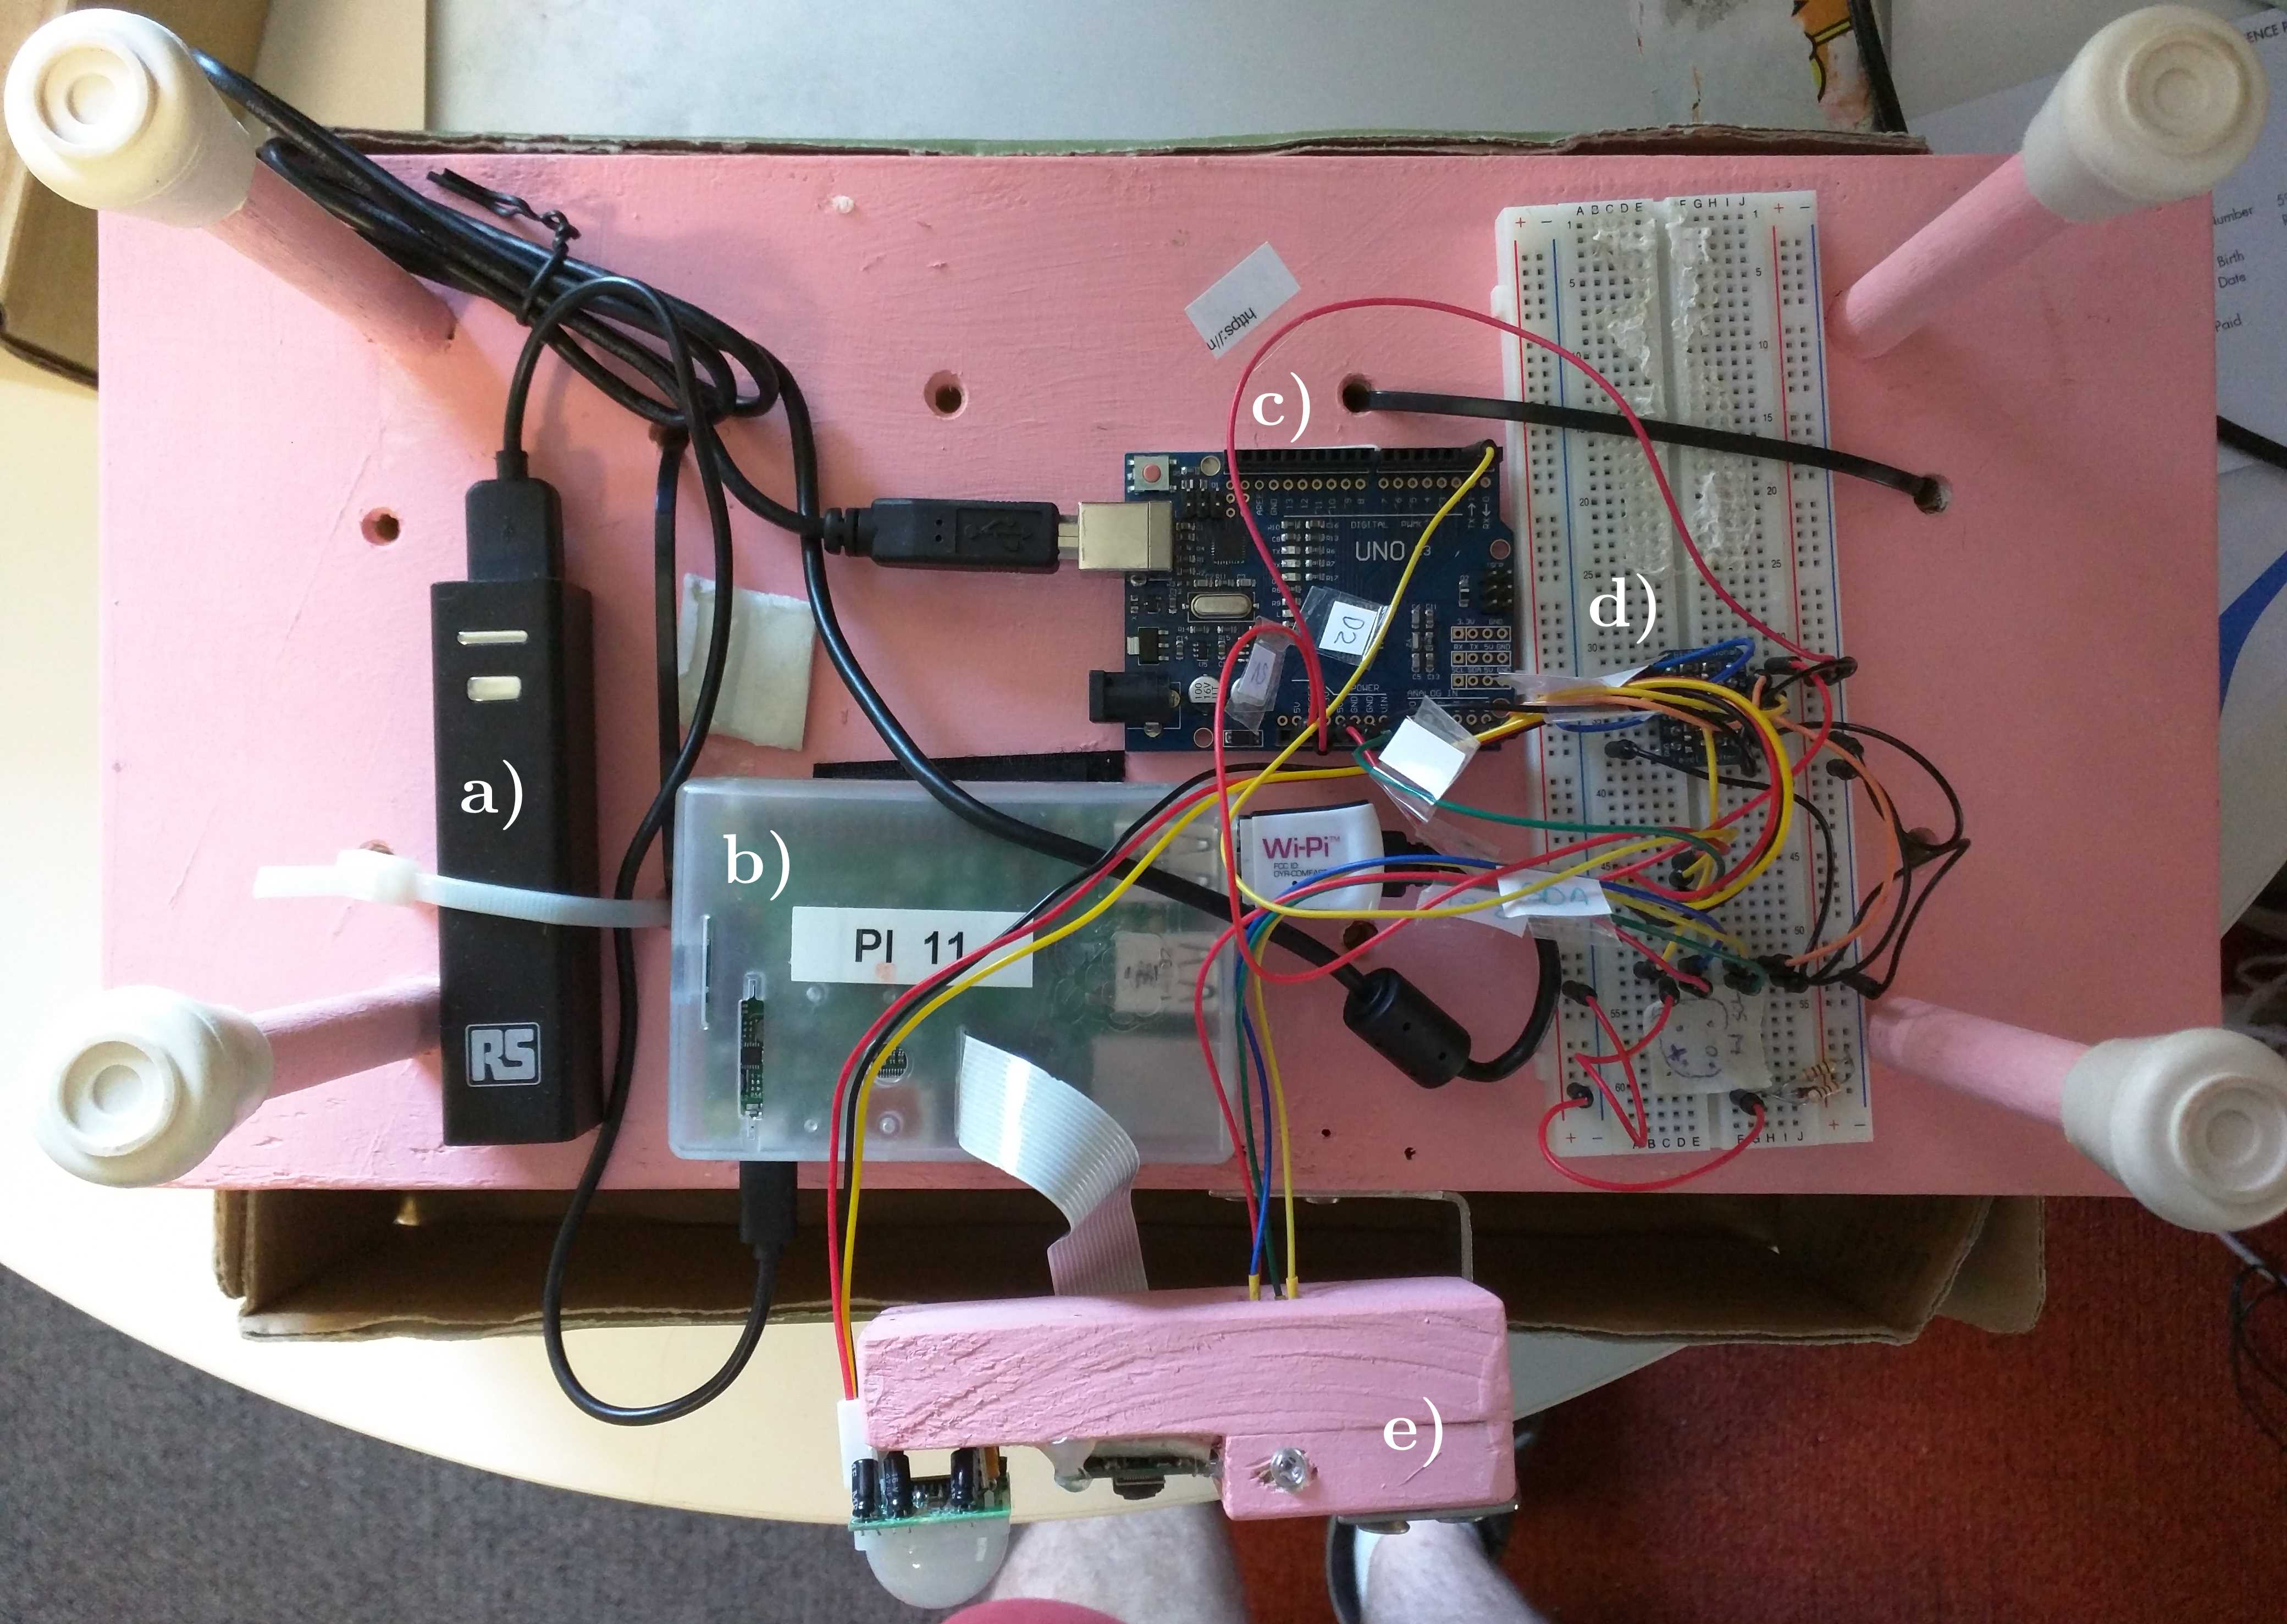
\includegraphics[width=\textwidth]{../diagrams/prototypeb-1.jpg}
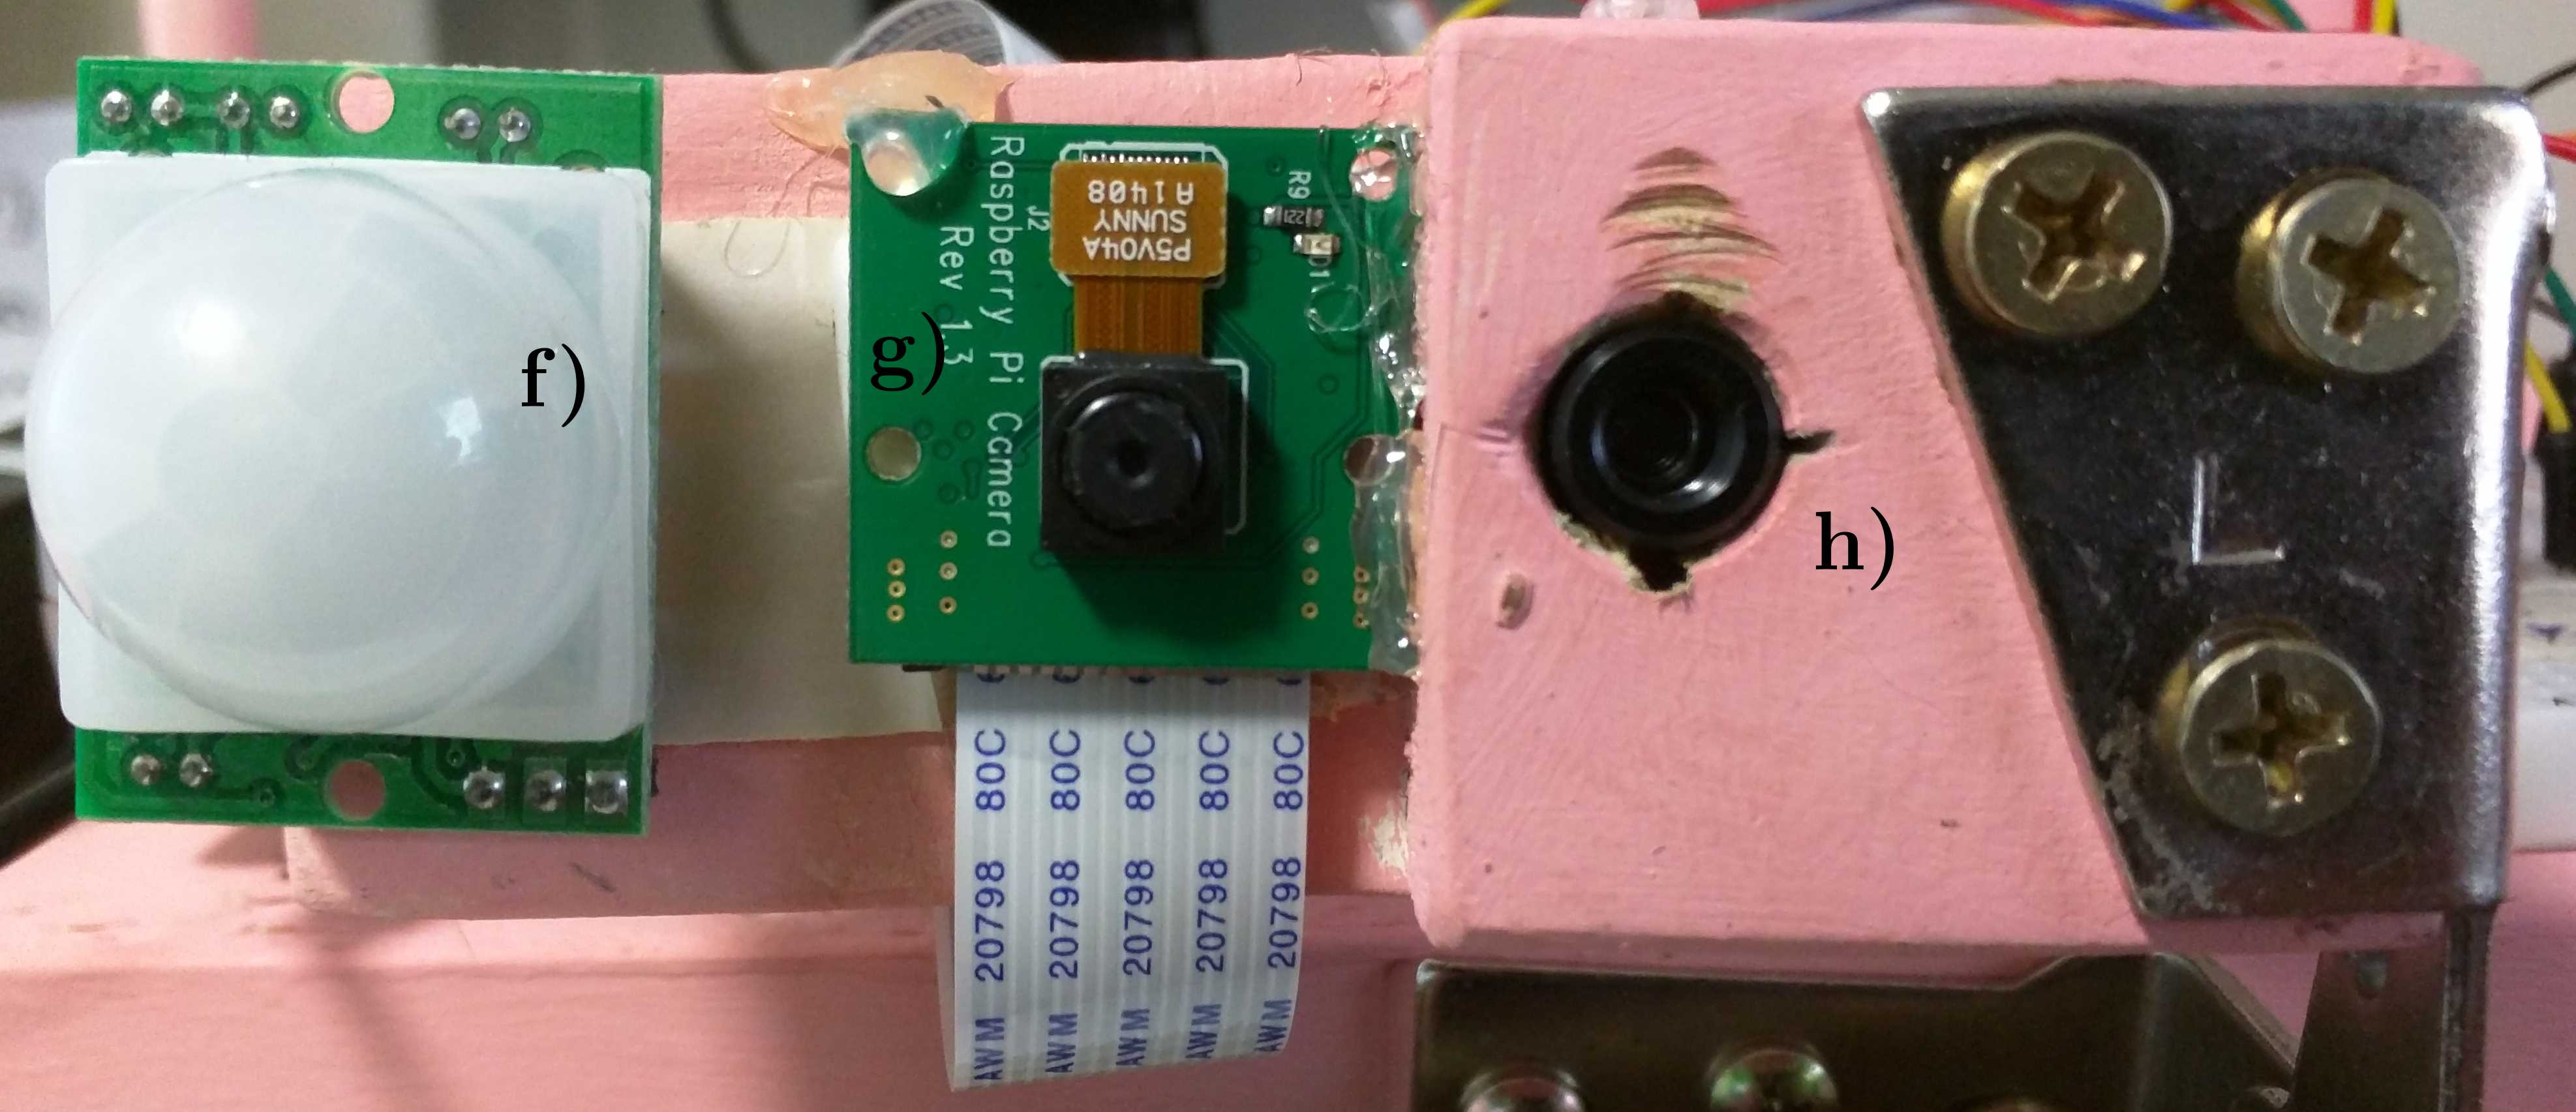
\includegraphics[width=\textwidth]{../diagrams/prototypeb-2.jpg}
{\small
\begin{multicols}{2}
\begin{enumerate}[a)]
 \item Battery pack
 \item Raspberry Pi
 \item Arduino
 \item Level-shifting circuitry
 \item Movable sensor mount
 \item PIR
 \item Camera
 \item \mlx
\end{enumerate}
\end{multicols}
}
\caption{Prototype B}
\label{fig:pictures:protob1}
\end{figure}

\begin{figure}
\centering
\begin{tikzpicture}[node distance=1.7cm]
\node (interwebs) [cbox] {Network};
\node (wifi) [dashbox, right=of interwebs] {\small WiFi / Ethernet};
\node (rpi) [fcont, below=of wifi] {Raspberry Pi \linebreak

  \tikz\node[fbox, minimum width=2.3cm, text width=2.3cm] {\small \ttfamily thinglib};
  \tikz\node[fbox, minimum width=2.3cm, text width=2.3cm] {\small \ttfamily features.py};
};
\node (cam) [box, right=of rpi] {Camera};
\node (usb) [dashbox, below=of rpi] {\small USB Serial};
\node (ard) [fcont, below=of usb] {Arduino \linebreak

  \tikz\node[fbox, minimum width=3.3cm, text width=3.3cm] {\small \ttfamily mlx90620\_driver};
};
\node (iic) [dashbox, left=of ard] {\small \iic};
\node (mlx) [box, below=of iic] {MLX90620};
\node (wire) [dashbox, right=of ard] {\small Interrupt};
\node (pir) [box, below=of wire] {PIR};

\draw [line] (interwebs) -- (wifi);
\draw [line] (wifi) -- (rpi);
\draw [line] (rpi) -- (usb);
\draw [line] (usb) -- (ard);
\draw [line] (ard) -- (iic);
\draw [line] (iic) -- (mlx);
\draw [line] (ard) -- (wire);
\draw [line] (wire) -- (pir);
\draw [line] (rpi) -- (cam);
\end{tikzpicture}
\caption{Prototype B system architecture}
\label{fig:pictures:protob-arch}
\end{figure}
 
 \ifcsdef{mainfile}{}{\bibliography{../references/primary}}
\end{document}
